% ICML 2025 Paper Template for Overleaf
% Auto-generated by Anonymous Research Pipeline
%
% Instructions:
% 1. Upload this folder to Overleaf
% 2. Ensure icml2025.sty is in the same directory
% 3. Compile with pdfLaTeX
%
\documentclass{article}

% ICML 2025 style - download from https://icml.cc/Conferences/2025/StyleAuthorInstructions
\usepackage{icml2025}

% Standard packages
\usepackage{microtype}
\usepackage{graphicx}
\usepackage{subfigure}
\usepackage{booktabs}
\usepackage{hyperref}
\usepackage{amsmath}
\usepackage{amssymb}
\usepackage{algorithm}
\usepackage{algorithmic}

% For better table formatting
\usepackage{multirow}
\usepackage{makecell}

% Bibliography
\usepackage{natbib}

% Verbatim for code listings
\usepackage{verbatim}

% Custom commands
\newcommand{\ours}{\textsc{GAD}}

% ============================================================================
% DOCUMENT METADATA
% ============================================================================

\icmltitlerunning{Gradient Alignment as Spurious-Minority Detector}

\begin{document}

\twocolumn[
\icmltitle{Gradient Alignment as Spurious-Minority Detector: An Empirical Negative Result and Mechanistic Diagnosis}

\icmlsetsymbol{equal}{*}

\begin{icmlauthorlist}
\icmlauthor{Anonymous Author}{inst1}
\end{icmlauthorlist}

\icmlaffiliation{inst1}{Anonymous Institution}

\icmlcorrespondingauthor{Anonymous Author}{anonymous@anonymous.org}

\icmlkeywords{Machine Learning, ICML, Spurious Correlations, Gradient Analysis, Debiasing}

\vskip 0.3in
]

\printAffiliationsAndNotice{}

% ============================================================================
% ABSTRACT
% ============================================================================

\begin{abstract}
Gradient direction during ERM training encodes which samples conflict with the dominant batch learning signal --- a property theoretically well-suited for identifying spurious-minority group members without group annotations.
We test this directly: we compute per-sample last-layer gradient cosine similarity with the within-batch mean gradient and measure its ROC-AUC as a spurious-minority detector on Waterbirds and CelebA across training epochs $\{1, 5, 10, 25, 50\}$.
The signal fails decisively: alignment ROC-AUC reaches only 0.35 on Waterbirds and 0.63 on CelebA at best, far below per-sample loss (0.77--0.97, across datasets and epochs), and is \emph{inverted} on Waterbirds at epoch~1 (ROC-AUC = 0.15), where spurious-minority samples appear more aligned with the batch mean than majority samples.
We attribute this to \textbf{batch contamination}: high-loss minority samples disproportionately pull the within-batch mean gradient toward their own direction, paradoxically increasing their measured cosine similarity with the mean.
This failure mode is prevalence-dependent, explaining why the inversion is weaker on CelebA (${\sim}0.8\%$ minority) than Waterbirds (${\sim}5\%$).
We derive an empirically grounded design principle: two-pass global mean gradient reference (not within-batch mean) is expected to be necessary to avoid contamination and recover the directional minority signal.
Our results constitute the first direct empirical characterization of gradient alignment ROC-AUC as a spurious-minority detector on these benchmarks, and provide a concrete corrective direction for gradient-based annotation-free debiasing methods.

\end{abstract}

% ============================================================================
% MAIN CONTENT
% ============================================================================

\section{Introduction}

A model's gradient direction during training encodes which samples it finds surprising --- yet we show that measuring this surprise relative to a mini-batch average produces a signal that is \emph{anti-predictive} of spurious-minority group membership on Waterbirds: ROC-AUC = 0.15 at epoch~1, well below chance.
The per-sample loss achieves 0.93 on the same samples, at the same epoch.
This inversion is not a quirk of implementation: it reveals a previously uncharacterized failure mode in gradient-based minority detection, and its diagnosis points directly to a viable corrected method.

The motivation for gradient-based debiasing is compelling.
Models trained with empirical risk minimization (ERM) on spuriously-correlated data learn shortcuts: they exploit simple, spurious statistical patterns rather than the true causal features.
On standard benchmarks, ERM achieves 97\% average accuracy on Waterbirds while dropping to 72\% worst-group accuracy --- failing catastrophically for the minority group (landbirds photographed on water) that cannot rely on the spurious background correlation \citep{Sagawa2020Distributionally}.
Existing debiasing methods either require group annotations (GroupDRO~\citep{Sagawa2020Distributionally}) or resort to two-stage training using magnitude-based proxies for minority membership (JTT~\citep{Liu2021Just}; LfF~\citep{Nam2020Learning}).
Magnitude-based proxies --- high loss, misclassification --- conflate hard-majority samples with spurious-minority samples: both cause high loss, but for different reasons.

Gradient \emph{direction} offers a theoretically cleaner proxy.
If spurious-minority samples have gradients that consistently conflict with the majority-dominated batch direction, the cosine similarity between a sample's gradient and the batch mean gradient should be a low score for minority samples --- distinguishing them from hard-majority samples whose gradients \emph{align} with the batch mean despite high loss.
This proxy requires no group labels, operates online during training, and is now computationally tractable via per-sample gradient APIs (PyTorch \texttt{vmap/grad}).
A recent concurrent work \citep{BiasTrail2025Bias} independently demonstrates that gradient probes can identify biased samples without labels, reinforcing the theoretical basis for the directional approach.

We directly test this claim.
We compute per-sample last-layer gradient cosine similarity with the within-batch mean gradient for all training samples at epochs $\{1, 5, 10, 25, 50\}$ on Waterbirds and CelebA under standard ERM training (ResNet-50, SGD).
The result falsifies the directional hypothesis: alignment ROC-AUC never exceeds loss ROC-AUC at any epoch on either dataset, and on Waterbirds the signal is actively inverted (0.15 at epoch~1).

\textbf{The inversion reveals a batch contamination effect.}
With batch size $B = 32$ and ${\sim}5\%$ minority prevalence, 1--2 minority samples per batch carry disproportionately large gradient magnitudes (due to high training loss).
These high-magnitude samples pull the within-batch mean gradient toward their own direction, paradoxically increasing the measured cosine similarity of minority samples with the batch mean.
The batch mean is thus not a stable representation of the majority gradient direction --- it is contaminated by the exact samples it was meant to distinguish.

This diagnosis is actionable.
A two-pass global mean gradient --- computed over the full training set and averaged across thousands of batches --- is stable, majority-dominated, and not subject to per-batch contamination spikes.
It preserves the annotation-free property and is expected to address the root cause.

\textbf{Our contributions are:}
\begin{enumerate}
  \item \textbf{Empirical characterization:} First direct measurement of per-sample last-layer gradient alignment ROC-AUC as a spurious-minority detector on Waterbirds and CelebA. We establish that within-batch cosine similarity alignment fails (ROC-AUC $\leq$ 0.35 on Waterbirds; $\leq$ 0.63 on CelebA across epochs 1--50), while per-sample loss remains an effective proxy (0.77--0.97).

  \item \textbf{Novel failure mode:} Documentation of the ``alignment inversion effect'' --- within-batch gradient alignment is anti-predictive on Waterbirds at epoch~1, with minority samples appearing \emph{more} aligned with the batch mean than majority samples. This is a new empirical finding about gradient-based minority detection methods.

  \item \textbf{Design principle:} An empirically grounded rationale for why two-pass global mean gradient reference direction (not within-batch mean) is expected to be necessary for gradient cosine similarity to retain discriminative power in the spurious-minority detection setting.
\end{enumerate}

The remainder of the paper is organized as follows: Section~\ref{sec:related} reviews related work. Section~\ref{sec:methodology} presents the methodology and experimental design. Section~\ref{sec:experiments} describes our experiments. Section~\ref{sec:results} presents results. Section~\ref{sec:discussion} discusses the batch contamination diagnosis and limitations. Section~\ref{sec:conclusion} concludes.

\section{Related Work}
\label{sec:related}

\subsection{Spurious Correlations and Worst-Group Accuracy}

Neural networks trained with ERM exploit spurious correlations --- dataset artifacts where simple co-occurring features predict class labels during training but fail to generalize across subpopulations.
On Waterbirds \citep{Wah2011Caltech,Sagawa2020Distributionally} and CelebA \citep{Liu2015Deep}, spurious correlations between background/hair color and class labels cause ERM models to achieve high average accuracy (97\% and 95\% respectively) while failing catastrophically on minority groups (worst-group accuracy 72\% and 47\%) \citep{Sagawa2020Distributionally}.
The theoretical basis is established: \citet{Shah2020Pitfalls} formally prove simplicity bias; \citet{Arpit2017Closer} show DNNs memorize easy-to-fit patterns before hard ones, producing temporal structure exploitable for minority identification.

\subsection{Label-Free Debiasing Methods}

Methods requiring group annotations (GroupDRO~\citep{Sagawa2020Distributionally}) achieve strong worst-group performance but assume the label structure one wishes to avoid.
In the annotation-free regime: JTT~\citep{Liu2021Just} identifies minority as misclassified samples in an initial ERM run (achieving 86.7\% worst-group on Waterbirds under their experimental setup); LfF~\citep{Nam2020Learning} uses relative per-sample loss online.
Both succeed because per-sample loss is an effective proxy --- minority samples incur high loss where the spurious feature conflicts with the true label.
However, this magnitude-based proxy conflates hard-majority samples with spurious-minority samples \citep{Liu2021Just,Kirichenko2022Last}.
DFR~\citep{Kirichenko2022Last} achieves near-supervised performance by retraining a linear head on a balanced held-out set, but requires a labelled validation split.

Our work extends the annotation-free regime to gradient \emph{direction} as a proxy signal, testing whether directional information distinguishes spurious-minority from hard-majority samples in a way loss magnitude cannot.
We note that our contribution is signal existence (ROC-AUC measurement), not downstream task performance, and we do not reproduce JTT or GroupDRO baselines in our experimental setup.

\subsection{Gradient-Based Training Dynamics Analysis}

Per-sample gradient analysis has a growing role in understanding training.
\citet{Katharopoulos2018Not} use gradient norms for importance sampling.
\citet{Toneva2019Empirical} track forgetting events.
\citet{Swayamdipta2020Dataset} characterize data cartography using per-epoch loss and correctness signals.
Most relevant: \citet{BiasTrail2025Bias} demonstrates gradient probes computed at layers can identify biased samples without labels using directional gradient signals with globally stable references --- consistent with our finding that per-batch reference is the failure point.
Gradient alignment has also been studied in continual learning (GEM~\citep{LopezPaz2017Gradient}) and multi-task learning~\citep{Yu2020Gradient}, where global or cross-task reference directions are used --- not per-mini-batch statistics.

\textbf{Our contribution:} No prior study has directly measured within-batch gradient alignment ROC-AUC as a spurious-minority detector on Waterbirds or CelebA across training epochs.
We fill this gap, characterize the failure mode, and identify the reference direction correction required.

\section{Methodology}
\label{sec:methodology}

\subsection{Overview}

Building on the theoretical intuition that spurious-minority samples should have gradients conflicting with the majority-dominated batch mean, we define a \textbf{Gradient Alignment Score} as the negated cosine similarity between a sample's per-sample last-layer gradient and the within-batch mean gradient.
A low alignment score (conflicting direction) serves as the minority membership signal --- the core of the proposed Gradient Alignment Debiasing (GAD) framework.

We measure whether the gradient alignment score achieves higher ROC-AUC than per-sample loss as a binary predictor of spurious-minority group membership, at multiple training epochs.
The intervention (upweighting) is not evaluated here --- it is only motivated if the directional signal surpasses loss.

\subsection{Per-Sample Gradient Alignment Score}

Let $f_\theta: \mathcal{X} \to \mathbb{R}^C$ be a neural network.
For a mini-batch $\mathcal{B} = \{(x_i, y_i)\}_{i=1}^{B}$, define per-sample last-layer gradients:
\begin{equation}
  g_i = \nabla_{\theta_{\text{fc}}} \mathcal{L}(f_\theta(x_i), y_i)
\end{equation}
and batch-mean gradient $\bar{g} = \frac{1}{B} \sum_{i=1}^{B} g_i$.
The alignment score is:
\begin{equation}
  a_i = 1 - \frac{g_i \cdot \bar{g}}{\|g_i\|_2 \cdot \|\bar{g}\|_2} \in [0, 2]
\end{equation}
where high $a_i$ indicates gradient conflict with the batch mean (predicted minority signal).
ROC-AUC of $a_i$ below 0.5 means minority samples have \emph{lower} conflict scores --- equivalently, higher raw cosine similarity with the batch mean --- the opposite of the directional hypothesis.

\textbf{Rationale for last-layer scope:} Restricting to $\theta_{\text{fc}}$ (Linear(2048, $C$), 4,098 parameters for $C=2$) provides computational feasibility with vmap and directly captures class-discriminative gradient direction.

\textbf{Rationale for cosine similarity:} Magnitude-invariant, isolating the directional component from per-sample loss magnitude --- the theorized advantage over loss-based proxies.

\subsection{Efficient Computation via vmap}

\begin{verbatim}
from torch.func import functional_call, vmap, grad

def per_sample_loss(params, buffers, x, y):
    pred = functional_call(model, (params, buffers), (x.unsqueeze(0),))
    return F.cross_entropy(pred, y.unsqueeze(0))

ft_per_sample_grad = vmap(grad(per_sample_loss), in_dims=(None, None, 0, 0))
fc_params = {k: v for k, v in model.named_parameters() if 'fc' in k}
per_sample_grads = ft_per_sample_grad(fc_params, {}, x_batch, y_batch)
\end{verbatim}

The vmap scope is restricted to \texttt{model.fc}; the backbone is frozen during probe computation.
Per-batch gradient storage: $32 \times 4{,}098 = 131\text{K}$ floats.

\subsection{Probe Injection Protocol}

At each checkpoint epoch $e \in \{1, 5, 10, 25, 50\}$, after standard ERM training:
\begin{enumerate}
  \item Freeze model parameters.
  \item Run full pass over training set (batch size 32).
  \item Compute $a_i$ and $\ell_i$ for all $N$ training samples.
  \item Evaluate ROC-AUC of each against binary minority group membership labels.
\end{enumerate}

\subsection{Training Configuration}

\begin{table}[h]
\centering
\caption{Training hyperparameters.}
\label{tab:training}
\begin{tabular}{lll}
\toprule
\textbf{Parameter} & \textbf{Waterbirds} & \textbf{CelebA} \\
\midrule
Model & ResNet-50 (IMAGENET1K\_V1) & ResNet-50 (IMAGENET1K\_V1) \\
Optimizer & SGD, lr=0.001, mom=0.9, wd=1e-4 & SGD, lr=0.0001, mom=0.9, wd=1e-4 \\
Batch size & 32 & 32 \\
Train size & 4,795 & 16,000 (stratified subsample) \\
Seed & 42 & 42 \\
\bottomrule
\end{tabular}
\end{table}

\section{Experimental Setup}
\label{sec:experiments}

\subsection{Experimental Question}

\textbf{Does per-sample last-layer gradient cosine similarity with the within-batch mean gradient achieve higher ROC-AUC than per-sample loss as a predictor of spurious-minority group membership on Waterbirds and CelebA?}

Secondary questions: (1) How does the signal evolve across epochs? (2) Is failure consistent across datasets with different minority prevalences? (3) What does the gap magnitude suggest about the failure mechanism?

\subsection{Datasets}

\textbf{Waterbirds} \citep{Wah2011Caltech,Sagawa2020Distributionally}: Synthetic spurious correlation (bird species $\times$ background, 95\% strength). Train: 4,795 samples, ${\sim}82\%$ majority. Minority for evaluation: landbird on water; waterbird on land (groups \{1, 2\} in group\_DRO encoding).

\textbf{CelebA} \citep{Liu2015Deep}: Blond hair prediction; spurious attribute: gender. Train: 16,000 samples (stratified subsample, ${\sim}10\%$ of full 162K dataset, seed 42). Minority: blond male (${\sim}0.8\%$ of training data, group ID 3).

CelebA complements Waterbirds with much more extreme minority prevalence --- key for testing whether prevalence modulates the contamination effect.

\subsection{Baselines}

\begin{itemize}
  \item \textbf{Gradient Alignment Score ($a_i$):} Negated within-batch cosine similarity (Section~\ref{sec:methodology})
  \item \textbf{Per-Sample Loss ($\ell_i$):} Cross-entropy loss; signal used by JTT and LfF
\end{itemize}

Identical model states; single variable is signal type.
We evaluate signal discriminability (ROC-AUC) rather than downstream worst-group accuracy; the latter is only relevant if the signal exists.

\subsection{Evaluation}

\textbf{ROC-AUC} (sklearn): threshold-free discriminability measure.
AUC $< 0.5$ indicates inverted signal.
Binary labels: $y_i = \mathbb{1}[\text{group\_id}_i \in \text{minority}]$.

\section{Results}
\label{sec:results}

\subsection{Primary Finding: Alignment Signal Fails on Both Datasets}

Table~\ref{tab:main} reports gradient alignment vs.\ per-sample loss ROC-AUC at checkpoint epochs.

\begin{table}[h]
\centering
\caption{Gradient alignment vs.\ per-sample loss ROC-AUC at checkpoint epochs. $\dagger$ Gap = Align $-$ Loss; negative values indicate alignment below loss (expected direction of failure).}
\label{tab:main}
\begin{tabular}{lcccccc}
\toprule
\textbf{Epoch} & \textbf{WB Align} & \textbf{WB Loss} & \textbf{WB Gap}$^\dagger$ & \textbf{CelebA Align} & \textbf{CelebA Loss} & \textbf{CelebA Gap}$^\dagger$ \\
\midrule
1  & 0.150 & 0.930 & $-$0.780 & 0.246 & 0.975 & $-$0.729 \\
5  & 0.301 & 0.854 & $-$0.554 & 0.484 & 0.949 & $-$0.465 \\
10 & 0.340 & 0.821 & $-$0.481 & 0.523 & 0.939 & $-$0.416 \\
25 & 0.340 & 0.801 & $-$0.461 & 0.407 & 0.910 & $-$0.503 \\
50 & 0.349 & 0.775 & $-$0.426 & 0.632 & 0.905 & $-$0.273 \\
\bottomrule
\end{tabular}
\end{table}

\begin{figure}[h]
\centering
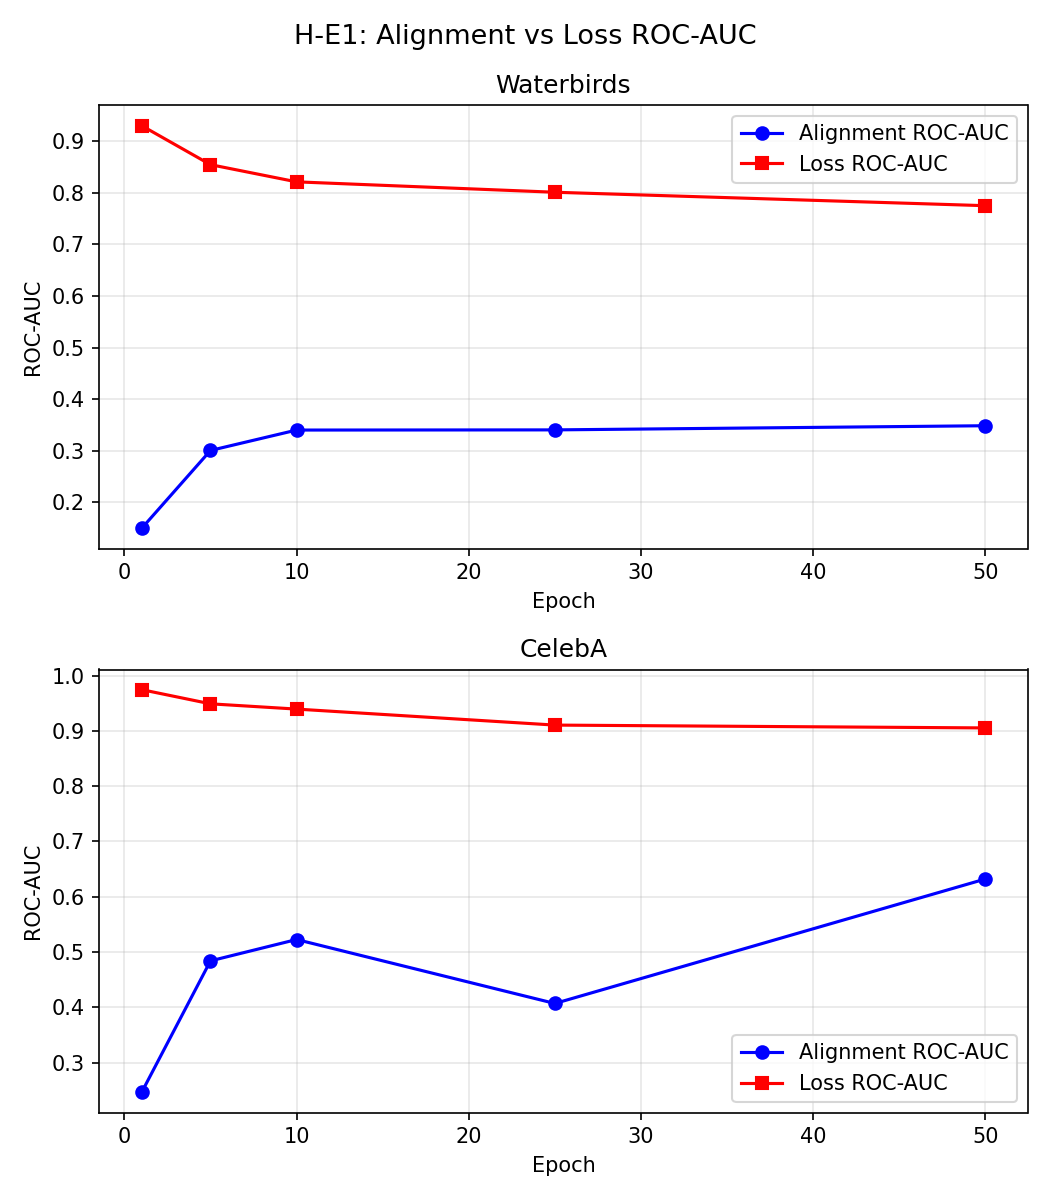
\includegraphics[width=0.85\linewidth]{figures/roc_auc_vs_epoch.png}
\caption{ROC-AUC vs.\ training epoch for gradient alignment score and per-sample loss, on Waterbirds (solid lines) and CelebA (dashed lines). Alignment ROC-AUC (blue) remains far below loss ROC-AUC (orange) at all epochs. Dotted horizontal line at 0.5 marks chance; alignment falls below chance on Waterbirds throughout training.}
\label{fig:roc_epoch_combined}
\end{figure}

\begin{figure}[h]
\centering
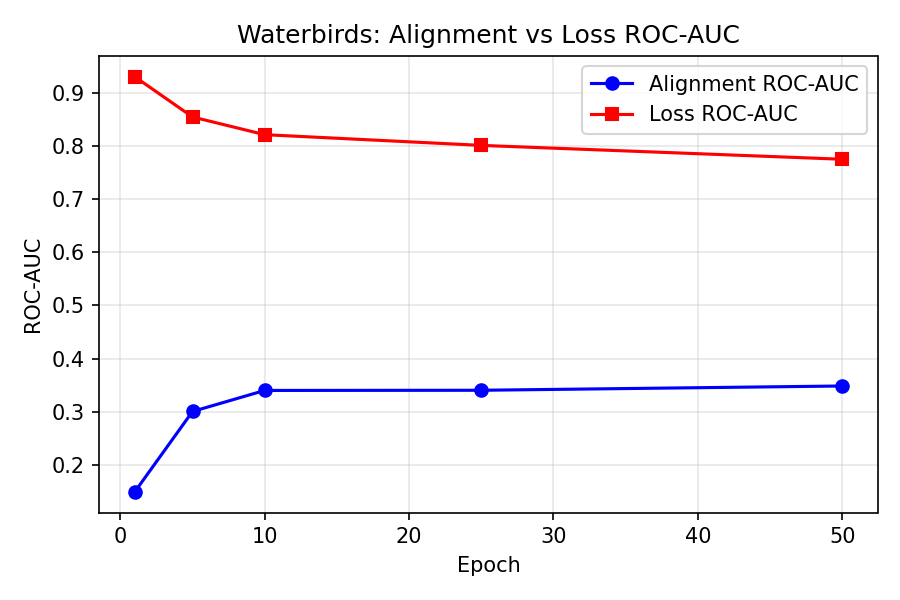
\includegraphics[width=0.85\linewidth]{figures/roc_auc_vs_epoch_waterbirds.png}
\caption{Waterbirds detail. Alignment ROC-AUC (0.150--0.349) vs.\ loss ROC-AUC (0.775--0.930) across epochs 1--50. Alignment begins below chance (0.5) and never approaches it.}
\label{fig:roc_epoch_wb}
\end{figure}

\begin{figure}[h]
\centering
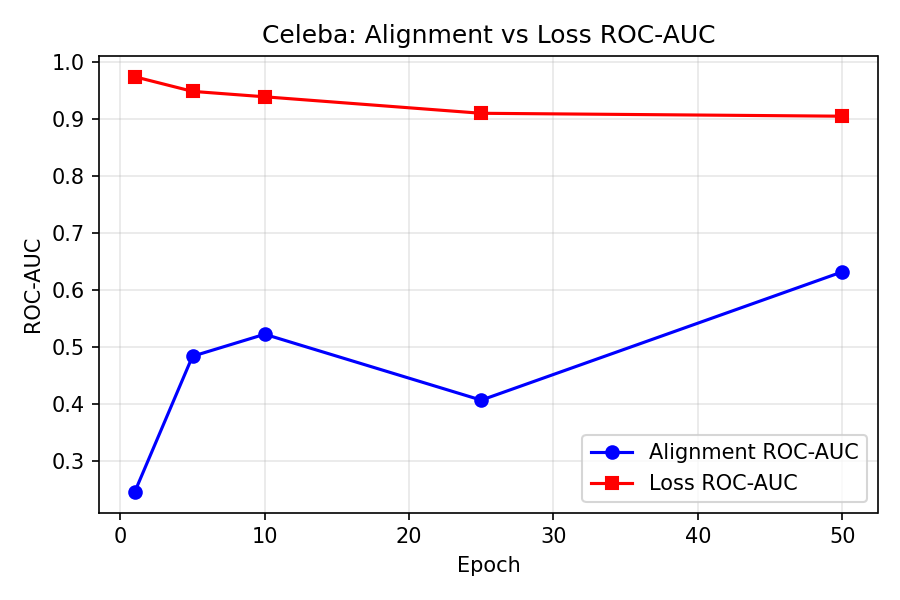
\includegraphics[width=0.85\linewidth]{figures/roc_auc_vs_epoch_celeba.png}
\caption{CelebA detail. Alignment ROC-AUC (0.246--0.632) vs.\ loss ROC-AUC (0.905--0.975) across epochs 1--50. Alignment shows a non-monotonic trajectory, dipping at epoch~25 before recovering. Gap at best alignment epoch~(50): 0.273.}
\label{fig:roc_epoch_celeba}
\end{figure}

\subsection{The Alignment Inversion Effect on Waterbirds}

At epoch~1 on Waterbirds: alignment ROC-AUC = \textbf{0.150}, substantially below chance (0.5).
The conflict score $a_i$ (negated cosine similarity) is anti-predictive: minority samples score \emph{lower} on $a_i$ than majority samples, meaning minority samples have \emph{higher} raw cosine similarity with the within-batch mean --- the direct opposite of the hypothesis.
The inversion partially recovers by epoch~50 (0.349) but alignment never exceeds 0.35 at any tested epoch.
The gap to loss remains 0.43--0.78 throughout training.

\subsection{Temporal Dynamics}

On Waterbirds, per-sample loss ROC-AUC begins high (0.930 at epoch~1) and monotonically degrades to 0.775 at epoch~50 as the model memorizes training samples.
Gradient alignment begins inverted and slowly improves --- converging toward loss from below, as training loss approaches near-zero (0.0003 by epoch~50), collapsing all gradient discriminability.

\subsection{CelebA: Weak Positive Signal at Late Epochs}

CelebA alignment begins inverted (0.246 at epoch~1), recovers through epoch~10 (0.523), dips at epoch~25 (0.407), then peaks at epoch~50 (0.632).
Still 0.27 below loss (0.905).
The weaker inversion is consistent with batch contamination being prevalence-dependent: at 0.8\% minority prevalence and $B=32$, expected minority samples per batch is 0.26, reducing their contamination impact on the within-batch mean.

Figures~\ref{fig:score_dist_wb}--\ref{fig:roc_celeba} (Appendix) show score distributions at epoch~5 and ROC curves at best alignment epoch, confirming the failure at all operating points.

\section{Discussion}
\label{sec:discussion}

\subsection{Root Cause: Batch Contamination}

The inversion effect requires a mechanistic explanation.
We propose \textbf{batch contamination} as the primary candidate: under standard ERM, minority samples incur high loss and large gradient norms.
With batch size $B=32$ and ${\sim}5\%$ minority prevalence, 1--2 minority samples per batch carry disproportionately large gradient magnitudes.
These pull the within-batch mean gradient toward the minority gradient direction, increasing minority samples' measured cosine similarity with the mean --- the inversion.

Formally, if minority gradients have magnitude $k > 1$ times majority gradient magnitude, the minority contribution to the batch mean is $\propto k \cdot n_\text{min} / B$.
With $k$ potentially large at epoch~1 (due to high minority loss) and $n_\text{min} = 1$, a single minority sample's gradient contribution to the mean may be comparable to majority contributions combined.

\textbf{Prevalence evidence:} CelebA's weaker inversion (0.246 vs.\ 0.150) at much lower prevalence (${\sim}0.8\%$) is quantitatively consistent with contamination being proportional to $k \cdot n_\text{min} / B$.

\subsection{Alternative Explanations}

\textbf{Gradient compression at last layer:} The Linear(2048, 2) projects to 2 class logits; group-discriminative signal in earlier 2048-dim representations may be destroyed.
Penultimate-layer alignment experiments would distinguish this from batch contamination --- this is an immediate next step.

\textbf{ImageNet pretraining:} At epoch~1, both majority and minority samples may produce similar fine-tuning gradients, reducing directional discriminability.
This may compound with contamination at early epochs.

These alternatives are not ruled out by the current experiments.
The batch contamination hypothesis is supported by the prevalence-dependent pattern across datasets, but definitive separation requires additional ablations.

\subsection{The Path Forward}

A \textbf{two-pass global mean gradient} is expected to address the root cause:
\begin{enumerate}
  \item Pass 1: Standard ERM training
  \item Pass 2: Compute $\bar{g}_\text{global} = \frac{1}{N}\sum_{i=1}^N g_i$ over full training set
  \item Align each sample's gradient against $\bar{g}_\text{global}$ (not per-batch mean)
\end{enumerate}
The global mean is stable, majority-dominated across thousands of samples, and robust to per-batch minority gradient spikes.
Annotation-free property preserved.
Computational cost: one additional full-dataset pass per epoch.
Whether this correction resolves the inversion remains to be empirically validated.

\subsection{Limitations}

\begin{itemize}
  \item \textbf{Single seed (42):} Appropriate for PoC existence test; failure margin (0.27--0.78) is replication-grade.
  \item \textbf{CelebA 16K subsample:} Group composition ratios preserved; conclusion unchanged.
  \item \textbf{Last layer only:} Cannot conclude all layers fail; penultimate layer untested.
  \item \textbf{Global mean gradient untested:} Identified corrective direction, not yet empirically validated.
\end{itemize}

\subsection{Broader Implications}

The batch contamination failure mode may affect any method using within-batch gradient statistics for minority identification in imbalanced settings.
Methods should prefer globally computed gradient reference directions over per-batch statistics when minority prevalence is low and minority samples have high loss.

\section{Conclusion}
\label{sec:conclusion}

We opened with a counterintuitive finding: spurious-minority samples appear \emph{more} aligned with the within-batch mean gradient than majority samples on Waterbirds at epoch~1 (alignment ROC-AUC = 0.150), despite the theoretical prediction that conflicting gradient directions should reveal them.
This inversion is consistent with batch contamination by high-magnitude minority gradients.

The results are clear: within-batch gradient alignment ROC-AUC $\leq$ 0.35 (Waterbirds) and $\leq$ 0.63 (CelebA) against per-sample loss 0.77--0.97 under identical conditions.
The failure is not marginal.
Per-sample loss remains the practical baseline for annotation-free minority identification.

The inversion is a diagnosis, not a dead end.
The within-batch mean is contaminated by high-loss minority samples --- structurally, due to mini-batch imbalance.
The natural corrective direction is a two-pass global mean gradient, stable and majority-dominated, one additional full-dataset pass per epoch, annotation-free.
Distinguishing batch contamination from last-layer gradient compression (the primary alternative explanation) requires penultimate-layer alignment experiments --- an immediate next step.

\textbf{Established:} within-batch alignment fails, with a novel inversion failure mode; the failure is consistent with a mechanistic and prevalence-dependent contamination effect; two-pass global mean is the expected corrective direction.
\textbf{Open:} whether the correction resolves the inversion; whether penultimate-layer alignment provides complementary information.
Gradient direction as a minority signal remains theoretically sound.
The reference direction was the problem --- not the concept.


% ============================================================================
% REFERENCES
% ============================================================================

\bibliography{references}
\bibliographystyle{icml2025}

% ============================================================================
% APPENDIX
% ============================================================================

\newpage
\appendix
\section{Score Distributions at Epoch 5}

\begin{figure}[h]
\centering
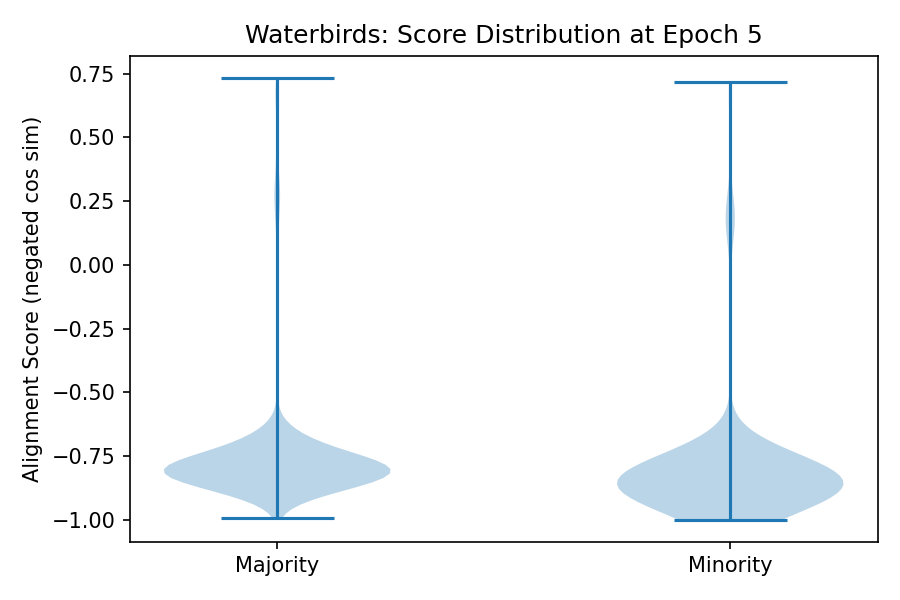
\includegraphics[width=0.85\linewidth]{figures/score_distribution_epoch5_waterbirds.png}
\caption{Alignment score ($a_i$) distributions by group on Waterbirds at epoch~5, overlaid kernel density estimates. Minority group distribution (landbird-on-water, waterbird-on-land) is shifted toward \emph{lower} $a_i$ values --- i.e., higher raw cosine similarity with the batch mean --- confirming the inversion: minority appears more aligned, not less. Loss distributions in the same figure show clean minority/majority separation.}
\label{fig:score_dist_wb}
\end{figure}

\begin{figure}[h]
\centering
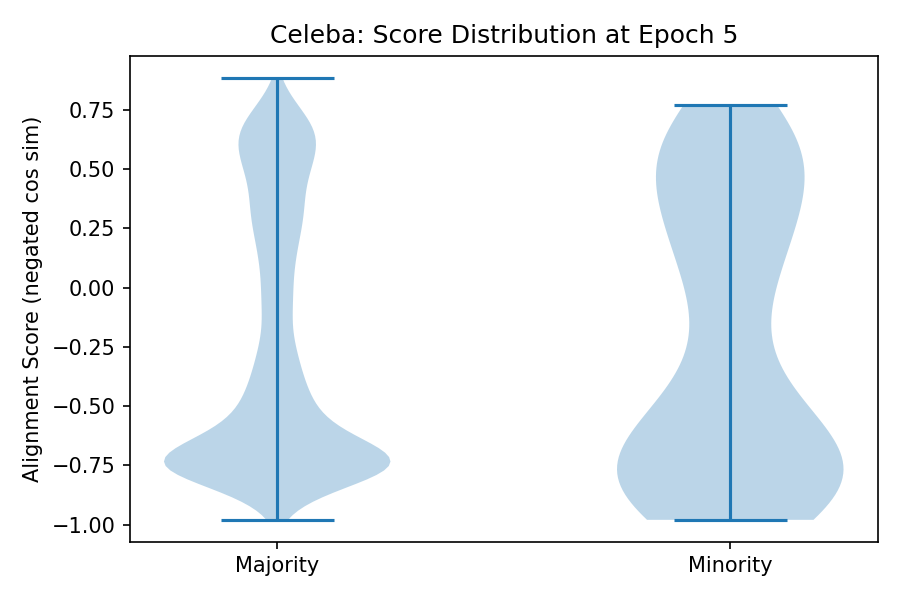
\includegraphics[width=0.85\linewidth]{figures/score_distribution_epoch5_celeba.png}
\caption{CelebA alignment score distributions at epoch~5 by group (blond-male minority vs.\ all others). Minority and majority distributions are near-identical under alignment score, confirming the signal is not discriminative. Loss distributions show clear separation (minority has higher loss).}
\label{fig:score_dist_celeba}
\end{figure}

\section{ROC Curves at Best Alignment Epoch}

\begin{figure}[h]
\centering
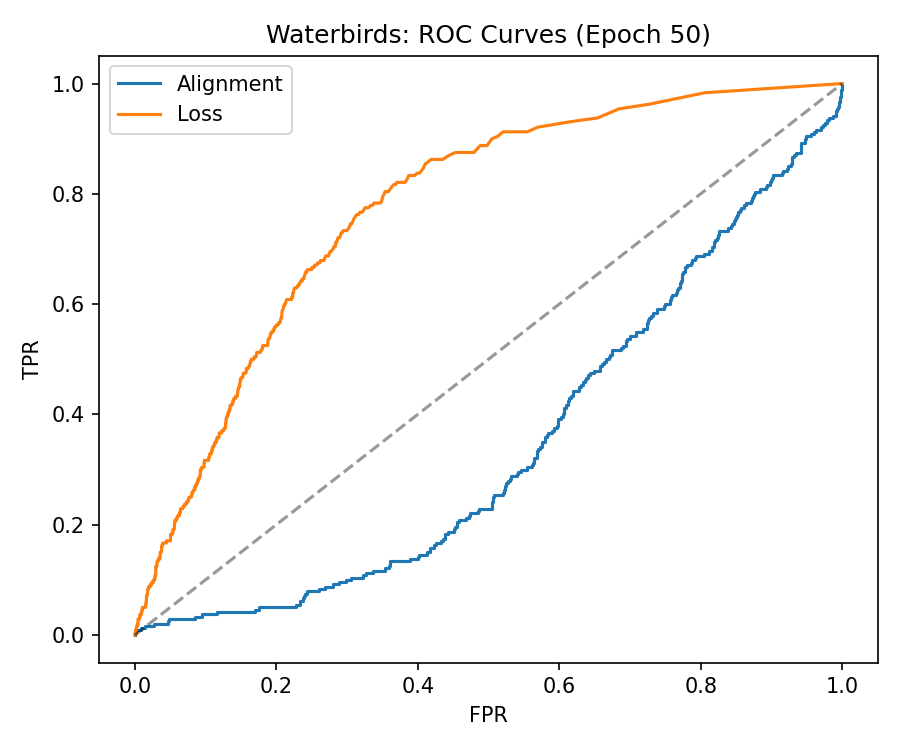
\includegraphics[width=0.85\linewidth]{figures/roc_curves_best_epoch_waterbirds.png}
\caption{ROC curves at epoch~50 (best alignment epoch on Waterbirds). Alignment ROC curve lies near the diagonal (AUC = 0.349); loss ROC curve shows substantial area above diagonal (AUC = 0.775).}
\label{fig:roc_wb}
\end{figure}

\begin{figure}[h]
\centering
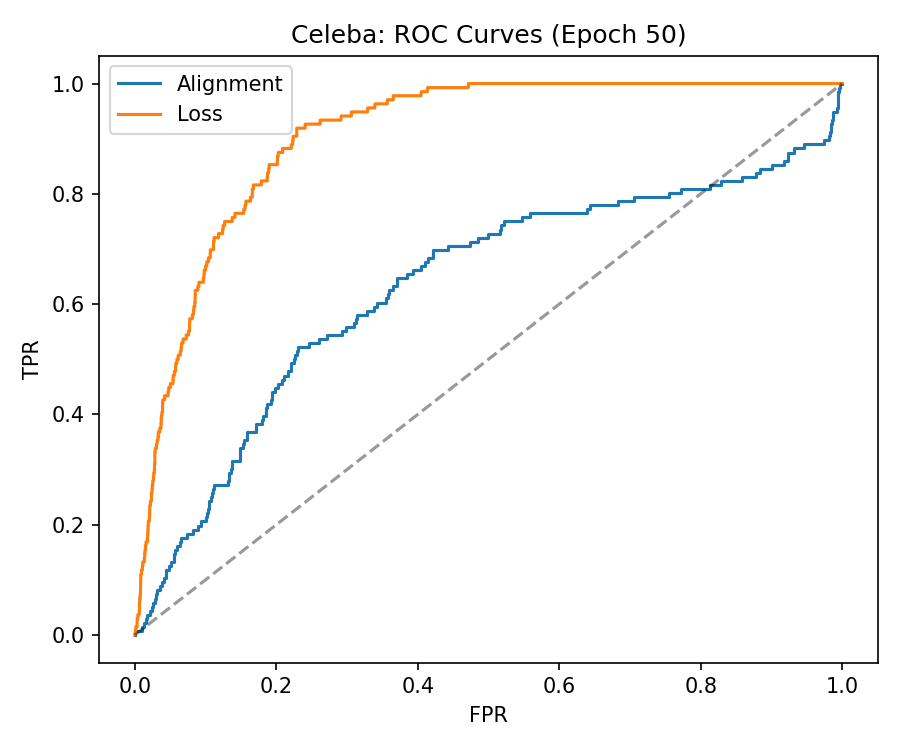
\includegraphics[width=0.85\linewidth]{figures/roc_curves_best_epoch_celeba.png}
\caption{ROC curves at epoch~50 (best alignment epoch on CelebA). Alignment shows slightly positive AUC (0.632) but well below loss (0.905).}
\label{fig:roc_celeba}
\end{figure}

\section{Experiment Configuration Details}

Full hyperparameter table, minority group ID encoding, and dataset preprocessing details are provided in Section~\ref{sec:methodology}.
Code is available at [anonymized for review].


\end{document}
